\documentclass{standalone}
\usepackage{tikz}
\usetikzlibrary{patterns}
\usetikzlibrary{positioning}
\usetikzlibrary{patterns, positioning}
\usetikzlibrary{shapes.misc}
\usepackage[outline]{contour}
\contourlength{1.5pt} 
\usetikzlibrary{calc}
        \usepackage{relsize}
        \tikzset{fontscale/.style = {font=\relsize{#1}}}

\begin{document}
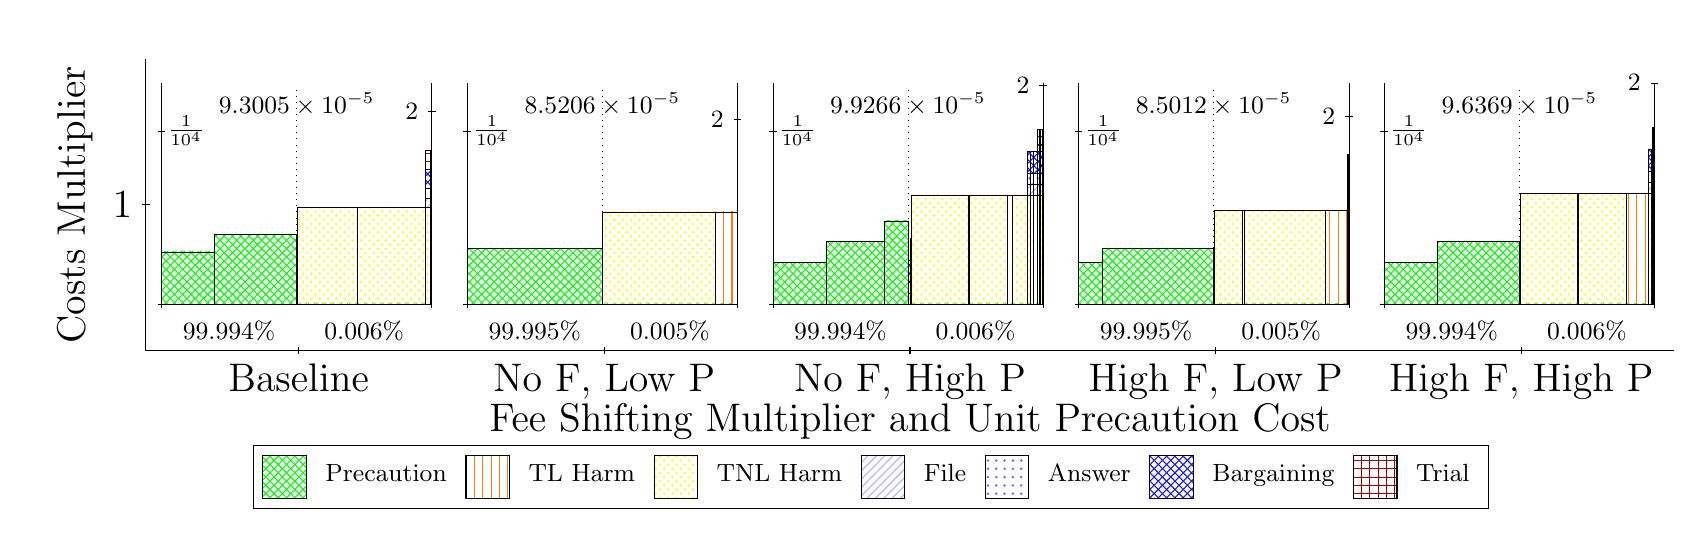
\begin{tikzpicture}
\clip(-0.5,-1.1) rectangle +(20.91,6.2);
\draw[black] (1,1) -- (1,4.7);
\node[rotate=90, fontscale=2, anchor=center] at (0.1, 2.85) {Costs Multiplier};
\draw[black] (0.95,2.85) -- (1.05,2.85);
\node[fontscale=2, anchor=east] at (0.95, 2.85) {1};

\draw[black] (1,1) -- (20.41,1);
\node[fontscale=2, anchor=center] at (10.705, 0.1) {Fee Shifting Multiplier and Unit Precaution Cost};
\draw[black] (2.941,0.95) -- (2.941,1.05);
\node[fontscale=2, anchor=north] at (2.941, 0.95) {Baseline};
\draw[black] (6.823,0.95) -- (6.823,1.05);
\node[fontscale=2, anchor=north] at (6.823, 0.95) {No F, Low P};
\draw[black] (10.705,0.95) -- (10.705,1.05);
\node[fontscale=2, anchor=north] at (10.705, 0.95) {No F, High P};
\draw[black] (14.587,0.95) -- (14.587,1.05);
\node[fontscale=2, anchor=north] at (14.587, 0.95) {High F, Low P};
\draw[black] (18.469,0.95) -- (18.469,1.05);
\node[fontscale=2, anchor=north] at (18.469, 0.95) {High F, High P};


\draw[pattern=crosshatch, pattern color=green,draw=black,very thin] (1.2,1.592) rectangle (1.8725,2.2513);
\draw[pattern=crosshatch, pattern color=green,draw=black,very thin] (1.8725,1.592) rectangle (2.916,2.4711);
\draw[pattern=crosshatch, pattern color=green,draw=black,very thin] (2.916,1.592) rectangle (2.9287,1.592);
\draw[pattern=north east lines, pattern color=blue!30,draw=black,very thin] (2.916,1.592) rectangle (2.9287,1.7142);
\draw[pattern=dots,  pattern color=blue!60,draw=black,very thin] (2.916,1.7142) rectangle (2.9287,1.8365);
\draw[pattern=crosshatch,      pattern color=blue!90,draw=black,very thin] (2.916,1.8365) rectangle (2.9287,2.0809);
\draw[pattern=grid,            pattern color=red!70!black,draw=black,very thin] (2.916,2.0809) rectangle (2.9287,2.3253);
\draw[pattern=crosshatch, pattern color=green,draw=black,very thin] (2.9287,1.592) rectangle (3.6818,1.592);
\draw[pattern=crosshatch dots, pattern color=yellow,draw=black,very thin] (2.9287,1.592) rectangle (3.6818,2.8141);
\draw[pattern=crosshatch, pattern color=green,draw=black,very thin] (3.6818,1.592) rectangle (3.6897,1.592);
\draw[pattern=vertical lines, pattern color=orange,draw=black,very thin] (3.6818,1.592) rectangle (3.6897,2.8141);
\draw[pattern=crosshatch, pattern color=green,draw=black,very thin] (3.6897,1.592) rectangle (4.5556,1.592);
\draw[pattern=crosshatch dots, pattern color=yellow,draw=black,very thin] (3.6897,1.592) rectangle (4.5556,2.8141);
\draw[pattern=crosshatch, pattern color=green,draw=black,very thin] (4.5556,1.592) rectangle (4.6122,1.592);
\draw[pattern=crosshatch dots, pattern color=yellow,draw=black,very thin] (4.5556,1.592) rectangle (4.6122,2.8141);
\draw[pattern=north east lines, pattern color=blue!30,draw=black,very thin] (4.5556,2.8141) rectangle (4.6122,2.9363);
\draw[pattern=dots,  pattern color=blue!60,draw=black,very thin] (4.5556,2.9363) rectangle (4.6122,3.0585);
\draw[pattern=crosshatch,      pattern color=blue!90,draw=black,very thin] (4.5556,3.0585) rectangle (4.6122,3.303);
\draw[pattern=grid,            pattern color=red!70!black,draw=black,very thin] (4.5556,3.303) rectangle (4.6122,3.5474);
\draw[pattern=crosshatch, pattern color=green,draw=black,very thin] (4.6122,1.592) rectangle (4.632,1.592);
\draw[pattern=vertical lines, pattern color=orange,draw=black,very thin] (4.6122,1.592) rectangle (4.632,2.8141);
\draw[pattern=north east lines, pattern color=blue!30,draw=black,very thin] (4.6122,2.8141) rectangle (4.632,2.9363);
\draw[pattern=dots,  pattern color=blue!60,draw=black,very thin] (4.6122,2.9363) rectangle (4.632,3.0585);
\draw[pattern=crosshatch,      pattern color=blue!90,draw=black,very thin] (4.6122,3.0585) rectangle (4.632,3.303);
\draw[pattern=grid,            pattern color=red!70!black,draw=black,very thin] (4.6122,3.303) rectangle (4.632,3.5474);
\node[font=\small,text=black,anchor=north] at (2.916, 4.4) {$9.3005\times 10^{-5}$};
\draw[black,very thin] (1.2,1.592) -- (1.2,4.4);
\draw[black,very thin] (1.15,1.592) -- (1.25,1.592);
\node[font=\small,text=black, anchor=west] at (1.15, 1.592) {};
\draw[black,very thin] (1.15,3.7897) -- (1.25,3.7897);
\node[font=\small,text=black, anchor=west] at (1.15, 3.7897) {$\frac{1}{10^{4}}$};

\draw[black,dotted,very thin] (2.916,1.6762) -- (2.916,4.3158);
\draw[black,very thin] (4.632,1.592) -- (4.632,4.4);
\draw[black,very thin] (4.582,4.0362) -- (4.682,4.0362);
\node[font=\small,text=black, anchor=east] at (4.582, 4.0362) {\contour{white}{2}};

\draw[black,very thin] (1.2,1.592) -- (4.632,1.592);
\draw[black,very thin] (1.2,1.542) -- (1.2,1.642);
\node[font=\small,text=black, anchor=north] at (1.2, 1.542) {};
\draw[black,very thin] (4.632,1.542) -- (4.632,1.642);
\node[font=\small,text=black, anchor=north] at (4.632, 1.542) {};

\node[font=\small,text=black,anchor=south] at (2.058, 0.992) {99.994\%};
\node[font=\small,text=black,anchor=south] at (3.774, 0.992) {0.006\%};

\draw[pattern=crosshatch, pattern color=green,draw=black,very thin] (5.082,1.592) rectangle (6.798,2.2953);
\draw[pattern=crosshatch, pattern color=green,draw=black,very thin] (6.798,1.592) rectangle (8.2353,1.592);
\draw[pattern=crosshatch dots, pattern color=yellow,draw=black,very thin] (6.798,1.592) rectangle (8.2353,2.7614);
\draw[pattern=crosshatch, pattern color=green,draw=black,very thin] (8.2353,1.592) rectangle (8.514,1.592);
\draw[pattern=vertical lines, pattern color=orange,draw=black,very thin] (8.2353,1.592) rectangle (8.514,2.7614);
\node[font=\small,text=black,anchor=north] at (6.798, 4.4) {$8.5206\times 10^{-5}$};
\draw[black,very thin] (5.082,1.592) -- (5.082,4.4);
\draw[black,very thin] (5.032,1.592) -- (5.132,1.592);
\node[font=\small,text=black, anchor=west] at (5.032, 1.592) {};
\draw[black,very thin] (5.032,3.7897) -- (5.132,3.7897);
\node[font=\small,text=black, anchor=west] at (5.032, 3.7897) {$\frac{1}{10^{4}}$};

\draw[black,dotted,very thin] (6.798,1.6762) -- (6.798,4.3158);
\draw[black,very thin] (8.514,1.592) -- (8.514,4.4);
\draw[black,very thin] (8.464,3.9308) -- (8.564,3.9308);
\node[font=\small,text=black, anchor=east] at (8.464, 3.9308) {\contour{white}{2}};

\draw[black,very thin] (5.082,1.592) -- (8.514,1.592);
\draw[black,very thin] (5.082,1.542) -- (5.082,1.642);
\node[font=\small,text=black, anchor=north] at (5.082, 1.542) {};
\draw[black,very thin] (8.514,1.542) -- (8.514,1.642);
\node[font=\small,text=black, anchor=north] at (8.514, 1.542) {};

\node[font=\small,text=black,anchor=south] at (5.94, 0.992) {99.995\%};
\node[font=\small,text=black,anchor=south] at (7.656, 0.992) {0.005\%};

\draw[pattern=crosshatch, pattern color=green,draw=black,very thin] (8.964,1.592) rectangle (9.6365,2.1194);
\draw[pattern=crosshatch, pattern color=green,draw=black,very thin] (9.6365,1.592) rectangle (10.378,2.3832);
\draw[pattern=crosshatch, pattern color=green,draw=black,very thin] (10.378,1.592) rectangle (10.68,2.6469);
\draw[pattern=crosshatch, pattern color=green,draw=black,very thin] (10.68,1.592) rectangle (10.687,1.592);
\draw[pattern=north east lines, pattern color=blue!30,draw=black,very thin] (10.68,1.592) rectangle (10.687,1.7306);
\draw[pattern=dots,  pattern color=blue!60,draw=black,very thin] (10.68,1.7306) rectangle (10.687,1.8691);
\draw[pattern=crosshatch,      pattern color=blue!90,draw=black,very thin] (10.68,1.8691) rectangle (10.687,2.1461);
\draw[pattern=crosshatch, pattern color=green,draw=black,very thin] (10.687,1.592) rectangle (10.704,1.592);
\draw[pattern=north east lines, pattern color=blue!30,draw=black,very thin] (10.687,1.592) rectangle (10.704,1.7306);
\draw[pattern=dots,  pattern color=blue!60,draw=black,very thin] (10.687,1.7306) rectangle (10.704,1.8691);
\draw[pattern=crosshatch,      pattern color=blue!90,draw=black,very thin] (10.687,1.8691) rectangle (10.704,2.1461);
\draw[pattern=crosshatch, pattern color=green,draw=black,very thin] (10.704,1.592) rectangle (10.708,1.592);
\draw[pattern=north east lines, pattern color=blue!30,draw=black,very thin] (10.704,1.592) rectangle (10.708,1.7306);
\draw[pattern=dots,  pattern color=blue!60,draw=black,very thin] (10.704,1.7306) rectangle (10.708,1.8691);
\draw[pattern=crosshatch,      pattern color=blue!90,draw=black,very thin] (10.704,1.8691) rectangle (10.708,2.1461);
\draw[pattern=grid,            pattern color=red!70!black,draw=black,very thin] (10.704,2.1461) rectangle (10.708,2.4232);
\draw[pattern=crosshatch, pattern color=green,draw=black,very thin] (10.708,1.592) rectangle (10.716,1.592);
\draw[pattern=north east lines, pattern color=blue!30,draw=black,very thin] (10.708,1.592) rectangle (10.716,1.7306);
\draw[pattern=dots,  pattern color=blue!60,draw=black,very thin] (10.708,1.7306) rectangle (10.716,1.8691);
\draw[pattern=crosshatch,      pattern color=blue!90,draw=black,very thin] (10.708,1.8691) rectangle (10.716,2.1461);
\draw[pattern=grid,            pattern color=red!70!black,draw=black,very thin] (10.708,2.1461) rectangle (10.716,2.4232);
\draw[pattern=crosshatch, pattern color=green,draw=black,very thin] (10.716,1.592) rectangle (11.451,1.592);
\draw[pattern=crosshatch dots, pattern color=yellow,draw=black,very thin] (10.716,1.592) rectangle (11.451,2.9773);
\draw[pattern=crosshatch, pattern color=green,draw=black,very thin] (11.451,1.592) rectangle (11.459,1.592);
\draw[pattern=vertical lines, pattern color=orange,draw=black,very thin] (11.451,1.592) rectangle (11.459,2.9773);
\draw[pattern=crosshatch, pattern color=green,draw=black,very thin] (11.459,1.592) rectangle (11.942,1.592);
\draw[pattern=crosshatch dots, pattern color=yellow,draw=black,very thin] (11.459,1.592) rectangle (11.942,2.9773);
\draw[pattern=crosshatch, pattern color=green,draw=black,very thin] (11.942,1.592) rectangle (12.003,1.592);
\draw[pattern=vertical lines, pattern color=orange,draw=black,very thin] (11.942,1.592) rectangle (12.003,2.9773);
\draw[pattern=crosshatch, pattern color=green,draw=black,very thin] (12.003,1.592) rectangle (12.192,1.5921);
\draw[pattern=crosshatch dots, pattern color=yellow,draw=black,very thin] (12.003,1.5921) rectangle (12.192,2.9773);
\draw[pattern=crosshatch, pattern color=green,draw=black,very thin] (12.192,1.592) rectangle (12.228,1.592);
\draw[pattern=crosshatch dots, pattern color=yellow,draw=black,very thin] (12.192,1.592) rectangle (12.228,2.9773);
\draw[pattern=north east lines, pattern color=blue!30,draw=black,very thin] (12.192,2.9773) rectangle (12.228,3.1158);
\draw[pattern=dots,  pattern color=blue!60,draw=black,very thin] (12.192,3.1158) rectangle (12.228,3.2543);
\draw[pattern=crosshatch,      pattern color=blue!90,draw=black,very thin] (12.192,3.2543) rectangle (12.228,3.5314);
\draw[pattern=crosshatch, pattern color=green,draw=black,very thin] (12.228,1.592) rectangle (12.238,1.592);
\draw[pattern=vertical lines, pattern color=orange,draw=black,very thin] (12.228,1.592) rectangle (12.238,2.9773);
\draw[pattern=north east lines, pattern color=blue!30,draw=black,very thin] (12.228,2.9773) rectangle (12.238,3.1158);
\draw[pattern=dots,  pattern color=blue!60,draw=black,very thin] (12.228,3.1158) rectangle (12.238,3.2543);
\draw[pattern=crosshatch,      pattern color=blue!90,draw=black,very thin] (12.228,3.2543) rectangle (12.238,3.5314);
\draw[pattern=crosshatch, pattern color=green,draw=black,very thin] (12.238,1.592) rectangle (12.266,1.592);
\draw[pattern=crosshatch dots, pattern color=yellow,draw=black,very thin] (12.238,1.592) rectangle (12.266,2.9773);
\draw[pattern=north east lines, pattern color=blue!30,draw=black,very thin] (12.238,2.9773) rectangle (12.266,3.1158);
\draw[pattern=dots,  pattern color=blue!60,draw=black,very thin] (12.238,3.1158) rectangle (12.266,3.2543);
\draw[pattern=crosshatch,      pattern color=blue!90,draw=black,very thin] (12.238,3.2543) rectangle (12.266,3.5314);
\draw[pattern=crosshatch, pattern color=green,draw=black,very thin] (12.266,1.592) rectangle (12.323,1.592);
\draw[pattern=vertical lines, pattern color=orange,draw=black,very thin] (12.266,1.592) rectangle (12.323,2.9773);
\draw[pattern=north east lines, pattern color=blue!30,draw=black,very thin] (12.266,2.9773) rectangle (12.323,3.1158);
\draw[pattern=dots,  pattern color=blue!60,draw=black,very thin] (12.266,3.1158) rectangle (12.323,3.2543);
\draw[pattern=crosshatch,      pattern color=blue!90,draw=black,very thin] (12.266,3.2543) rectangle (12.323,3.5314);
\draw[pattern=crosshatch, pattern color=green,draw=black,very thin] (12.323,1.592) rectangle (12.347,1.592);
\draw[pattern=crosshatch dots, pattern color=yellow,draw=black,very thin] (12.323,1.592) rectangle (12.347,2.9773);
\draw[pattern=north east lines, pattern color=blue!30,draw=black,very thin] (12.323,2.9773) rectangle (12.347,3.1158);
\draw[pattern=dots,  pattern color=blue!60,draw=black,very thin] (12.323,3.1158) rectangle (12.347,3.2543);
\draw[pattern=crosshatch,      pattern color=blue!90,draw=black,very thin] (12.323,3.2543) rectangle (12.347,3.5314);
\draw[pattern=grid,            pattern color=red!70!black,draw=black,very thin] (12.323,3.5314) rectangle (12.347,3.8084);
\draw[pattern=crosshatch, pattern color=green,draw=black,very thin] (12.347,1.592) rectangle (12.356,1.592);
\draw[pattern=vertical lines, pattern color=orange,draw=black,very thin] (12.347,1.592) rectangle (12.356,2.9773);
\draw[pattern=north east lines, pattern color=blue!30,draw=black,very thin] (12.347,2.9773) rectangle (12.356,3.1158);
\draw[pattern=dots,  pattern color=blue!60,draw=black,very thin] (12.347,3.1158) rectangle (12.356,3.2543);
\draw[pattern=crosshatch,      pattern color=blue!90,draw=black,very thin] (12.347,3.2543) rectangle (12.356,3.5314);
\draw[pattern=grid,            pattern color=red!70!black,draw=black,very thin] (12.347,3.5314) rectangle (12.356,3.8084);
\draw[pattern=crosshatch, pattern color=green,draw=black,very thin] (12.356,1.592) rectangle (12.381,1.592);
\draw[pattern=crosshatch dots, pattern color=yellow,draw=black,very thin] (12.356,1.592) rectangle (12.381,2.9773);
\draw[pattern=north east lines, pattern color=blue!30,draw=black,very thin] (12.356,2.9773) rectangle (12.381,3.1158);
\draw[pattern=dots,  pattern color=blue!60,draw=black,very thin] (12.356,3.1158) rectangle (12.381,3.2543);
\draw[pattern=crosshatch,      pattern color=blue!90,draw=black,very thin] (12.356,3.2543) rectangle (12.381,3.5314);
\draw[pattern=grid,            pattern color=red!70!black,draw=black,very thin] (12.356,3.5314) rectangle (12.381,3.8084);
\draw[pattern=crosshatch, pattern color=green,draw=black,very thin] (12.381,1.592) rectangle (12.396,1.592);
\draw[pattern=vertical lines, pattern color=orange,draw=black,very thin] (12.381,1.592) rectangle (12.396,2.9773);
\draw[pattern=north east lines, pattern color=blue!30,draw=black,very thin] (12.381,2.9773) rectangle (12.396,3.1158);
\draw[pattern=dots,  pattern color=blue!60,draw=black,very thin] (12.381,3.1158) rectangle (12.396,3.2543);
\draw[pattern=crosshatch,      pattern color=blue!90,draw=black,very thin] (12.381,3.2543) rectangle (12.396,3.5314);
\draw[pattern=grid,            pattern color=red!70!black,draw=black,very thin] (12.381,3.5314) rectangle (12.396,3.8084);
\node[font=\small,text=black,anchor=north] at (10.68, 4.4) {$9.9266\times 10^{-5}$};
\draw[black,very thin] (8.964,1.592) -- (8.964,4.4);
\draw[black,very thin] (8.914,1.592) -- (9.014,1.592);
\node[font=\small,text=black, anchor=west] at (8.914, 1.592) {};
\draw[black,very thin] (8.914,3.7897) -- (9.014,3.7897);
\node[font=\small,text=black, anchor=west] at (8.914, 3.7897) {$\frac{1}{10^{4}}$};

\draw[black,dotted,very thin] (10.68,1.6762) -- (10.68,4.3158);
\draw[black,very thin] (12.396,1.592) -- (12.396,4.4);
\draw[black,very thin] (12.346,4.3625) -- (12.446,4.3625);
\node[font=\small,text=black, anchor=east] at (12.346, 4.3625) {\contour{white}{2}};

\draw[black,very thin] (8.964,1.592) -- (12.396,1.592);
\draw[black,very thin] (8.964,1.542) -- (8.964,1.642);
\node[font=\small,text=black, anchor=north] at (8.964, 1.542) {};
\draw[black,very thin] (12.396,1.542) -- (12.396,1.642);
\node[font=\small,text=black, anchor=north] at (12.396, 1.542) {};

\node[font=\small,text=black,anchor=south] at (9.822, 0.992) {99.994\%};
\node[font=\small,text=black,anchor=south] at (11.538, 0.992) {0.006\%};

\draw[pattern=crosshatch, pattern color=green,draw=black,very thin] (12.846,1.592) rectangle (13.148,2.1195);
\draw[pattern=crosshatch, pattern color=green,draw=black,very thin] (13.148,1.592) rectangle (14.562,2.2953);
\draw[pattern=crosshatch, pattern color=green,draw=black,very thin] (14.562,1.592) rectangle (14.565,1.592);
\draw[pattern=north east lines, pattern color=blue!30,draw=black,very thin] (14.562,1.592) rectangle (14.565,1.7109);
\draw[pattern=dots,  pattern color=blue!60,draw=black,very thin] (14.562,1.7109) rectangle (14.565,1.8298);
\draw[pattern=crosshatch,      pattern color=blue!90,draw=black,very thin] (14.562,1.8298) rectangle (14.565,2.0676);
\draw[pattern=grid,            pattern color=red!70!black,draw=black,very thin] (14.562,2.0676) rectangle (14.565,2.3054);
\draw[pattern=crosshatch, pattern color=green,draw=black,very thin] (14.565,1.592) rectangle (14.931,1.592);
\draw[pattern=crosshatch dots, pattern color=yellow,draw=black,very thin] (14.565,1.592) rectangle (14.931,2.7811);
\draw[pattern=crosshatch, pattern color=green,draw=black,very thin] (14.931,1.592) rectangle (14.947,1.592);
\draw[pattern=vertical lines, pattern color=orange,draw=black,very thin] (14.931,1.592) rectangle (14.947,2.7811);
\draw[pattern=crosshatch, pattern color=green,draw=black,very thin] (14.947,1.592) rectangle (15.985,1.592);
\draw[pattern=crosshatch dots, pattern color=yellow,draw=black,very thin] (14.947,1.592) rectangle (15.985,2.7811);
\draw[pattern=crosshatch, pattern color=green,draw=black,very thin] (15.985,1.592) rectangle (16.259,1.592);
\draw[pattern=vertical lines, pattern color=orange,draw=black,very thin] (15.985,1.592) rectangle (16.259,2.7811);
\draw[pattern=crosshatch, pattern color=green,draw=black,very thin] (16.259,1.592) rectangle (16.269,1.592);
\draw[pattern=crosshatch dots, pattern color=yellow,draw=black,very thin] (16.259,1.592) rectangle (16.269,2.7811);
\draw[pattern=north east lines, pattern color=blue!30,draw=black,very thin] (16.259,2.7811) rectangle (16.269,2.9);
\draw[pattern=dots,  pattern color=blue!60,draw=black,very thin] (16.259,2.9) rectangle (16.269,3.0189);
\draw[pattern=crosshatch,      pattern color=blue!90,draw=black,very thin] (16.259,3.0189) rectangle (16.269,3.2567);
\draw[pattern=grid,            pattern color=red!70!black,draw=black,very thin] (16.259,3.2567) rectangle (16.269,3.4945);
\draw[pattern=crosshatch, pattern color=green,draw=black,very thin] (16.269,1.592) rectangle (16.278,1.592);
\draw[pattern=vertical lines, pattern color=orange,draw=black,very thin] (16.269,1.592) rectangle (16.278,2.7811);
\draw[pattern=north east lines, pattern color=blue!30,draw=black,very thin] (16.269,2.7811) rectangle (16.278,2.9);
\draw[pattern=dots,  pattern color=blue!60,draw=black,very thin] (16.269,2.9) rectangle (16.278,3.0189);
\draw[pattern=crosshatch,      pattern color=blue!90,draw=black,very thin] (16.269,3.0189) rectangle (16.278,3.2567);
\draw[pattern=grid,            pattern color=red!70!black,draw=black,very thin] (16.269,3.2567) rectangle (16.278,3.4945);
\node[font=\small,text=black,anchor=north] at (14.562, 4.4) {$8.5012\times 10^{-5}$};
\draw[black,very thin] (12.846,1.592) -- (12.846,4.4);
\draw[black,very thin] (12.796,1.592) -- (12.896,1.592);
\node[font=\small,text=black, anchor=west] at (12.796, 1.592) {};
\draw[black,very thin] (12.796,3.7897) -- (12.896,3.7897);
\node[font=\small,text=black, anchor=west] at (12.796, 3.7897) {$\frac{1}{10^{4}}$};

\draw[black,dotted,very thin] (14.562,1.6762) -- (14.562,4.3158);
\draw[black,very thin] (16.278,1.592) -- (16.278,4.4);
\draw[black,very thin] (16.228,3.9701) -- (16.328,3.9701);
\node[font=\small,text=black, anchor=east] at (16.228, 3.9701) {\contour{white}{2}};

\draw[black,very thin] (12.846,1.592) -- (16.278,1.592);
\draw[black,very thin] (12.846,1.542) -- (12.846,1.642);
\node[font=\small,text=black, anchor=north] at (12.846, 1.542) {};
\draw[black,very thin] (16.278,1.542) -- (16.278,1.642);
\node[font=\small,text=black, anchor=north] at (16.278, 1.542) {};

\node[font=\small,text=black,anchor=south] at (13.704, 0.992) {99.995\%};
\node[font=\small,text=black,anchor=south] at (15.42, 0.992) {0.005\%};

\draw[pattern=crosshatch, pattern color=green,draw=black,very thin] (16.728,1.592) rectangle (17.4,2.1194);
\draw[pattern=crosshatch, pattern color=green,draw=black,very thin] (17.4,1.592) rectangle (18.444,2.3832);
\draw[pattern=crosshatch, pattern color=green,draw=black,very thin] (18.444,1.592) rectangle (18.45,1.592);
\draw[pattern=north east lines, pattern color=blue!30,draw=black,very thin] (18.444,1.592) rectangle (18.45,1.7324);
\draw[pattern=dots,  pattern color=blue!60,draw=black,very thin] (18.444,1.7324) rectangle (18.45,1.8728);
\draw[pattern=crosshatch,      pattern color=blue!90,draw=black,very thin] (18.444,1.8728) rectangle (18.45,2.1536);
\draw[pattern=crosshatch, pattern color=green,draw=black,very thin] (18.45,1.592) rectangle (18.455,1.592);
\draw[pattern=north east lines, pattern color=blue!30,draw=black,very thin] (18.45,1.592) rectangle (18.455,1.7324);
\draw[pattern=dots,  pattern color=blue!60,draw=black,very thin] (18.45,1.7324) rectangle (18.455,1.8728);
\draw[pattern=crosshatch,      pattern color=blue!90,draw=black,very thin] (18.45,1.8728) rectangle (18.455,2.1536);
\draw[pattern=grid,            pattern color=red!70!black,draw=black,very thin] (18.45,2.1536) rectangle (18.455,2.4344);
\draw[pattern=crosshatch, pattern color=green,draw=black,very thin] (18.455,1.592) rectangle (19.18,1.592);
\draw[pattern=crosshatch dots, pattern color=yellow,draw=black,very thin] (18.455,1.592) rectangle (19.18,2.996);
\draw[pattern=crosshatch, pattern color=green,draw=black,very thin] (19.18,1.592) rectangle (19.188,1.592);
\draw[pattern=vertical lines, pattern color=orange,draw=black,very thin] (19.18,1.592) rectangle (19.188,2.996);
\draw[pattern=crosshatch, pattern color=green,draw=black,very thin] (19.188,1.592) rectangle (19.797,1.5921);
\draw[pattern=crosshatch dots, pattern color=yellow,draw=black,very thin] (19.188,1.5921) rectangle (19.797,2.996);
\draw[pattern=crosshatch, pattern color=green,draw=black,very thin] (19.797,1.592) rectangle (20.082,1.5921);
\draw[pattern=vertical lines, pattern color=orange,draw=black,very thin] (19.797,1.5921) rectangle (20.082,2.996);
\draw[pattern=crosshatch, pattern color=green,draw=black,very thin] (20.082,1.592) rectangle (20.117,1.592);
\draw[pattern=crosshatch dots, pattern color=yellow,draw=black,very thin] (20.082,1.592) rectangle (20.117,2.996);
\draw[pattern=north east lines, pattern color=blue!30,draw=black,very thin] (20.082,2.996) rectangle (20.117,3.1364);
\draw[pattern=dots,  pattern color=blue!60,draw=black,very thin] (20.082,3.1364) rectangle (20.117,3.2768);
\draw[pattern=crosshatch,      pattern color=blue!90,draw=black,very thin] (20.082,3.2768) rectangle (20.117,3.5576);
\draw[pattern=crosshatch, pattern color=green,draw=black,very thin] (20.117,1.592) rectangle (20.127,1.592);
\draw[pattern=vertical lines, pattern color=orange,draw=black,very thin] (20.117,1.592) rectangle (20.127,2.996);
\draw[pattern=north east lines, pattern color=blue!30,draw=black,very thin] (20.117,2.996) rectangle (20.127,3.1364);
\draw[pattern=dots,  pattern color=blue!60,draw=black,very thin] (20.117,3.1364) rectangle (20.127,3.2768);
\draw[pattern=crosshatch,      pattern color=blue!90,draw=black,very thin] (20.117,3.2768) rectangle (20.127,3.5576);
\draw[pattern=crosshatch, pattern color=green,draw=black,very thin] (20.127,1.592) rectangle (20.151,1.592);
\draw[pattern=crosshatch dots, pattern color=yellow,draw=black,very thin] (20.127,1.592) rectangle (20.151,2.996);
\draw[pattern=north east lines, pattern color=blue!30,draw=black,very thin] (20.127,2.996) rectangle (20.151,3.1364);
\draw[pattern=dots,  pattern color=blue!60,draw=black,very thin] (20.127,3.1364) rectangle (20.151,3.2768);
\draw[pattern=crosshatch,      pattern color=blue!90,draw=black,very thin] (20.127,3.2768) rectangle (20.151,3.5576);
\draw[pattern=grid,            pattern color=red!70!black,draw=black,very thin] (20.127,3.5576) rectangle (20.151,3.8384);
\draw[pattern=crosshatch, pattern color=green,draw=black,very thin] (20.151,1.592) rectangle (20.16,1.592);
\draw[pattern=vertical lines, pattern color=orange,draw=black,very thin] (20.151,1.592) rectangle (20.16,2.996);
\draw[pattern=north east lines, pattern color=blue!30,draw=black,very thin] (20.151,2.996) rectangle (20.16,3.1364);
\draw[pattern=dots,  pattern color=blue!60,draw=black,very thin] (20.151,3.1364) rectangle (20.16,3.2768);
\draw[pattern=crosshatch,      pattern color=blue!90,draw=black,very thin] (20.151,3.2768) rectangle (20.16,3.5576);
\draw[pattern=grid,            pattern color=red!70!black,draw=black,very thin] (20.151,3.5576) rectangle (20.16,3.8384);
\node[font=\small,text=black,anchor=north] at (18.444, 4.4) {$9.6369\times 10^{-5}$};
\draw[black,very thin] (16.728,1.592) -- (16.728,4.4);
\draw[black,very thin] (16.678,1.592) -- (16.778,1.592);
\node[font=\small,text=black, anchor=west] at (16.678, 1.592) {};
\draw[black,very thin] (16.678,3.7897) -- (16.778,3.7897);
\node[font=\small,text=black, anchor=west] at (16.678, 3.7897) {$\frac{1}{10^{4}}$};

\draw[black,dotted,very thin] (18.444,1.6762) -- (18.444,4.3158);
\draw[black,very thin] (20.16,1.592) -- (20.16,4.4);
\draw[black,very thin] (20.11,4.4) -- (20.21,4.4);
\node[font=\small,text=black, anchor=east] at (20.11, 4.4) {\contour{white}{2}};

\draw[black,very thin] (16.728,1.592) -- (20.16,1.592);
\draw[black,very thin] (16.728,1.542) -- (16.728,1.642);
\node[font=\small,text=black, anchor=north] at (16.728, 1.542) {};
\draw[black,very thin] (20.16,1.542) -- (20.16,1.642);
\node[font=\small,text=black, anchor=north] at (20.16, 1.542) {};

\node[font=\small,text=black,anchor=south] at (17.586, 0.992) {99.994\%};
\node[font=\small,text=black,anchor=south] at (19.302, 0.992) {0.006\%};

\coordinate (LegendAnchor) at (10.205000000000002,0);
\begin{scope}[align=center]
\matrix[scale=0.6,draw=black,below=0.2cm of LegendAnchor,nodes={draw},column sep=0.12cm]{
\node[rectangle,draw,minimum width=0.55cm,minimum height=0.55cm,pattern=crosshatch, pattern color=green]{}; &
        \node[draw=none,font=\small]{Precaution}; &
\node[rectangle,draw,minimum width=0.55cm,minimum height=0.55cm,pattern=vertical lines, pattern color=orange]{}; &
        \node[draw=none,font=\small]{TL Harm}; &
\node[rectangle,draw,minimum width=0.55cm,minimum height=0.55cm,pattern=crosshatch dots, pattern color=yellow]{}; &
        \node[draw=none,font=\small]{TNL Harm}; &
\node[rectangle,draw,minimum width=0.55cm,minimum height=0.55cm,pattern=north east lines, pattern color=blue!30]{}; &
        \node[draw=none,font=\small]{File}; &
\node[rectangle,draw,minimum width=0.55cm,minimum height=0.55cm,pattern=dots, pattern color=blue!60]{}; &
        \node[draw=none,font=\small]{Answer}; &
\node[rectangle,draw,minimum width=0.55cm,minimum height=0.55cm,pattern=crosshatch, pattern color=blue!90]{}; &
        \node[draw=none,font=\small]{Bargaining}; &
\node[rectangle,draw,minimum width=0.55cm,minimum height=0.55cm,pattern=grid, pattern color=red!70!black]{}; &
        \node[draw=none,font=\small]{Trial}; \\
};\end{scope}

\end{tikzpicture}
\end{document}